% Title: gl2ps_renderer figure
% Creator: GL2PS 1.4.0, (C) 1999-2017 C. Geuzaine
% For: Octave
% CreationDate: Thu Nov 28 12:47:56 2019
\setlength{\unitlength}{1pt}
\begin{picture}(0,0)
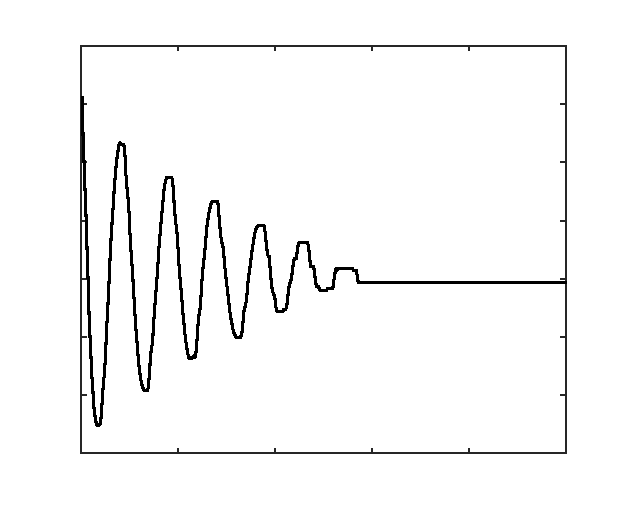
\includegraphics{../Report/img/lego-inc}
\end{picture}%
\begin{picture}(300,250)(0,0)
\fontsize{10}{0}
\selectfont\put(39,25){\makebox(0,0)[t]{\textcolor[rgb]{0.15,0.15,0.15}{{0}}}}
\fontsize{10}{0}
\selectfont\put(85.5,25){\makebox(0,0)[t]{\textcolor[rgb]{0.15,0.15,0.15}{{100}}}}
\fontsize{10}{0}
\selectfont\put(132,25){\makebox(0,0)[t]{\textcolor[rgb]{0.15,0.15,0.15}{{200}}}}
\fontsize{10}{0}
\selectfont\put(178.5,25){\makebox(0,0)[t]{\textcolor[rgb]{0.15,0.15,0.15}{{300}}}}
\fontsize{10}{0}
\selectfont\put(225,25){\makebox(0,0)[t]{\textcolor[rgb]{0.15,0.15,0.15}{{400}}}}
\fontsize{10}{0}
\selectfont\put(271.5,25){\makebox(0,0)[t]{\textcolor[rgb]{0.15,0.15,0.15}{{500}}}}
\fontsize{10}{0}
\selectfont\put(34.0107,32.4815){\makebox(0,0)[r]{\textcolor[rgb]{0.15,0.15,0.15}{{-1.5}}}}
\fontsize{10}{0}
\selectfont\put(34.0107,60.4128){\makebox(0,0)[r]{\textcolor[rgb]{0.15,0.15,0.15}{{-1}}}}
\fontsize{10}{0}
\selectfont\put(34.0107,88.344){\makebox(0,0)[r]{\textcolor[rgb]{0.15,0.15,0.15}{{-0.5}}}}
\fontsize{10}{0}
\selectfont\put(34.0107,116.275){\makebox(0,0)[r]{\textcolor[rgb]{0.15,0.15,0.15}{{0}}}}
\fontsize{10}{0}
\selectfont\put(34.0107,144.206){\makebox(0,0)[r]{\textcolor[rgb]{0.15,0.15,0.15}{{0.5}}}}
\fontsize{10}{0}
\selectfont\put(34.0107,172.138){\makebox(0,0)[r]{\textcolor[rgb]{0.15,0.15,0.15}{{1}}}}
\fontsize{10}{0}
\selectfont\put(34.0107,200.069){\makebox(0,0)[r]{\textcolor[rgb]{0.15,0.15,0.15}{{1.5}}}}
\fontsize{10}{0}
\selectfont\put(34.0107,228){\makebox(0,0)[r]{\textcolor[rgb]{0.15,0.15,0.15}{{2}}}}
\fontsize{11}{0}
\selectfont\put(155.25,12){\makebox(0,0)[t]{\textcolor[rgb]{0.15,0.15,0.15}{{Tiempo}}}}
\fontsize{11}{0}
\selectfont\put(11.0107,130.241){\rotatebox{90}{\makebox(0,0)[b]{\textcolor[rgb]{0.15,0.15,0.15}{{$\theta$}}}}}
\fontsize{11}{0}
\selectfont\put(155.25,238){\makebox(0,0)[b]{\textcolor[rgb]{0,0,0}{{Posición angular del péndulo}}}}
\end{picture}
